\documentclass[11pt,aspectratio=43]{beamer}
\usepackage[utf8]{inputenc}
\usepackage{amsmath, amsfonts, amssymb, amsthm}
\usepackage[T1]{fontenc}
\usepackage{lmodern}
\usepackage{xcolor}
\usepackage{setspace}
\usepackage{booktabs}
\usepackage{multirow}
\usepackage{graphicx}
\usepackage{tikz}
% \usetikzlibrary{decorations}
\usetikzlibrary{decorations.pathreplacing}
\usepackage{ulem}
\usepackage{hyperref}
\usepackage{booktabs}
\usepackage{babel}
\usepackage{makecell}
\usepackage[para,online,flushleft]{threeparttable}
\usepackage{pdfpages}
\usepackage{tcolorbox}
\usepackage{bm}
\usepackage{appendixnumberbeamer}
\usepackage{natbib}
\usepackage{caption}
\captionsetup[figure]{labelformat=empty}% redefines the caption setup of the figures environment in the beamer class.
\usetheme[compress]{Boadilla}
\usecolortheme{default}
\useoutertheme{miniframes}
\usefonttheme[onlymath]{serif}

\newcommand{\jump}[2]{\hyperlink{#1}{\beamerbutton{#2}}}
\newcommand{\orange}[1]{\textcolor{orange}{#1}}
\newcommand{\red}[1]{\textcolor{red}{#1}}

\setbeamertemplate{itemize item}{\raisebox{0.1em}{\scalebox{0.7}{$\blacksquare$}}}
\setbeamertemplate{itemize subitem}[circle]
\setbeamertemplate{itemize subsubitem}{--}
\setbeamercolor{itemize item}{fg=black}
\setbeamercolor{itemize subitem}{fg=black}
\setbeamercolor{itemize subsubitem}{fg=black}
\setbeamercolor{item projected}{bg=darkgray,fg=white}
\definecolor{blue}{rgb}{0.2, 0.2, 0.7}
\setbeamercolor{alerted text}{fg=blue}
\setbeamertemplate{enumerate items}[circle]


\setbeamertemplate{headline}{}

%==========================================
\let\olditemize=\itemize
\let\endolditemize=\enditemize
\renewenvironment{itemize}{\olditemize \itemsep1em}{\endolditemize}
\let\oldenumerate=\enumerate
\let\endoldenumerate=\endenumerate
\renewenvironment{enumerate}{\oldenumerate \itemsep1em}{ \endoldenumerate}

\DeclareMathOperator*{\argmax}{\arg\!\max}
\DeclareMathOperator*{\E}{\mathbb{E}}
\DeclareMathOperator*{\var}{\rm Var}
\DeclareMathOperator*{\cov}{\rm Cov}

\theoremstyle{definition}
\newtheorem{assume}{Assumption}
\newtheorem{lem}{Lemma}
\newtheorem{proposition}{Proposition}
\newtheorem{thm}{Theorem}
\newtheorem{corol}{Corollary}

\begin{document}
    \title[Lecture 14]{Lecture 14 \\ The Real Business Cycle Model \\ Part 1: Consumer}
    \author[Hui-Jun Chen]{Hui-Jun Chen}
    \institute[OSU]{The Ohio State University}
    % \date{\today}
    \date{\today}
    \setbeamertemplate{navigation symbols}{}
    \setstretch{1.2}

%-------------------------------------------------------
{
%	\usebackgroundtemplate{\includegraphics[width=1\paperwidth]{../EveningSky_cropped_edit43_bright.jpg}}
    \begin{frame}
% \vspace{3em}
        \centering
%		{\footnotesize 	ECON 4002 Intermediate Macroeconomic Theory}
        \maketitle
% \vspace{-1.5em}
% \centering
% \includegraphics[width=0.55\linewidth]{Pictures/houses.jpeg}


    \end{frame}
}

% -------------------------------------------
\setbeamertemplate{headline}
{
\setbeamercolor{section in head/foot}{fg=black, bg=white}
\vskip1em \tiny \insertsectionnavigationhorizontal{1\paperwidth}{\hspace{0.70\paperwidth}}{}
}
%------------------------------------------

\begin{frame}{Overview}
\label{slide:Overview}
    \begin{itemize}
        \item Recall that in Lecture 13, there is no production in dynamic model.
        \item The following $ 5 $ lectures is for \textbf{Real Business Cycle} (RBC) model:
        \begin{itemize}
            \item Lecture 14: consumer
            \item Lecture 15: firm
            \item Lecture 16: competitive equilibrium
            \item Lecture 17: formal example
            \item Lecture 18: application to bring RBC to data
        \end{itemize}
    \end{itemize}
\end{frame}

\begin{frame}{Real Business Cycle Model}
\label{slide:Real_Business_Cycle_Model}
\begin{itemize}
    \item One of the workhorse frameworks in modern macroecnomics
    \item \alert{Real}: not about \textit{money} and \textit{inflation}
    \item \alert{Business Cycle}: mainly explain the short- and medium-term economics fluctuation (``business cycle frequency'')
    \item Three agents: representative consumer, representative firm, and government
    \item All agents make \textbf{static and dynamic} decisions
    \item Larger ``scale'' model (i.e., more endogenous variables), but build upon the technique learned before
\end{itemize}
\end{frame}

\section{Consumer}
\label{sec:Consumer}

\begin{frame}{Consumer: Constraints}
\label{slide:Consumer__Constraints}
There are \alert{$ 11 $} variables associated with the representative consumer:
\begin{itemize}
    \item choice variables: consumption ($C, C'$) and labor supply ($N_{S}, N'_{S}$)
    \begin{itemize}
        \item leisure follows labor choice: $ l = h - N_{S} $, and $ l' = h - N'_{S} $
    \end{itemize}
    \item owns the firm and get profits ($ \pi, \pi' $) and pays taxes ($T, T'$)
    \item taken the equilibrium price as given ($w, w', r$)
\end{itemize}
%
Saving ($S$) at date 0 to construct lifetime budget constraint:
\begin{align*}
    \text{today:} \quad
        & C + S = w N_{S} + \pi - T
    \\
    \text{tomorrow:} \quad
        & C' = w' N_{S}' + \pi' - T' + ( 1+r ) S
    \\
    \text{lifetime constraint:} \quad
        & C + \frac{C'}{1+r} =
            \underbrace{w N_{S} + \pi - T}_{\approx Y \text{ in last lecture}}
            + \frac{\overbrace{w' N'_{S} + \pi' - T'}^{\approx Y' \text{ in last lecture}}}{1+r}
\end{align*}
%
\end{frame}

\begin{frame}{Consumer: Preference}
\label{slide:Consumer__Preference}
    In general, utility fcn across consumption and labor choice can be mixed:
    \begin{itemize}
        \item e.g. mix $ C $ and $ N_{S} $: \alert{\href{https://tinyurl.com/222w66m9}{GHH preferences}}
        \item e.g. mix current and future: \alert{\href{https://tinyurl.com/2p8a9bb5}{Epstein–Zin preferences}}
    \end{itemize}
    Here, we are making simplified assumption: \textbf{additive for both direction}:
    %
    \begin{equation}
    \label{eq:utility_function}
        U( C, C', N_{S}, N'_{S} ) = u( C ) - v( N_{S}) + u( C' ) - v( N'_{S} )
    .\end{equation}
    %
    To see why \alert{additive} can simplify analysis, recall the MRS in both \alert{intratemporal} (w/i period) and \alert{intertemporal} (b/w period) substitution:
    %
    \begin{equation*}
        MRS_{l, C} = - MRS_{N_{S}, C} = \frac{v'( N_{S} )}{u'( C )}, \text{and } MRS_{C, C'} = \frac{u'( C )}{u'( C' )}
    .\end{equation*}
    %
\end{frame}

\begin{frame}{Representative Consumer's Problem}
\label{slide:Representative_Consumer_s_Problem}
%
\begin{equation}
\label{eq:consumer_problem}
    \begin{split}
        \max_{C, C', N_{S}, N'_{S}} \quad
            & u( C ) - v( N_{S}) + u( C' ) - v( N'_{S} )
        \\
        \text{subject to } \quad
            & C + \frac{C'}{1+r} =
            w N_{S} + \pi - T
            + \frac{w' N'_{S} + \pi' - T'}{1+r}
        \\
    \end{split}
.\end{equation}
%
\begin{itemize}
    \item Hard to analyze in graph, $ \because $ $ 4 $ choices variables $ \Rightarrow  $ $ 4 $-dim problem!
    \item Yet, usual procedure in Calculus still works!
    \item Why? Because \alert{partial derivatives} only looks the optimality in \alert{$ 1 $-dim}
    \item Each FOC is optimal for $ 1 $-dim $ \Rightarrow  $ solution satisfies ALL FOCs
\end{itemize}
\end{frame}

\begin{frame}{Consumer's Optimality Conditions}
\label{slide:Consumer_s_Optimality_Conditions}
\begin{itemize}
    \item Step 1: substitute $ C $ by budget constraint,
        %
        \begin{align*}
            \max_{C', N_{S}, N'_{S}}
                & u\left(
                    w N_{S} + \pi - T + \frac{w' N'_{S} + \pi' - T' - C'}{1+r}
                   \right)
            \\
                & - v( N_{S} ) + u( C' ) - v( N'_{S} )
        \end{align*}
        %
    \item Step 2: find FOCs for $ C', N_{S} $, and $ N'_{S} $:
    %
    \begin{align*}
        [C']: \quad
            & u'( C' ) - \frac{1}{1+r}u'( C ) = 0 \Rightarrow u'( C' ) = \frac{1}{1+r} u'( C )
        \\
        [ N_{S} ]: \quad
            & w u'( C ) - v'( N_{S} ) = 0 \Rightarrow w u'( C ) = v'( N_{S} )
        \\
        [ N'_{S} ]: \quad
            & \frac{w'}{1+r} u'( C ) - v'( N'_{S} ) = 0 \Rightarrow \frac{w'}{1+r} u'( C ) = v'( N'_{S} )
    \end{align*}
    %
\end{itemize}
\end{frame}

\begin{frame}{Consumer's Optimality Conditions (Cont.)}
\label{slide:Consumer_s_Optimality_Conditions__Cont__}
    \begin{itemize}
        \item Step 3: Compute multiple MRSs:
        %
        \begin{align*}
            [C']: \quad
                & MRS_{C, C'} = \frac{u'( C )}{u'( C' )} = 1+r
            \\
            [ N_{S} ]: \quad
                & -MRS_{N_{S}, C} = MRS_{l, C} = \frac{v'( N_{S} )}{u'( C )} = w
            \\
            [ N'_{S} ]: \quad
                & MRS_{l', C} = \frac{v'( N'_{S} )}{u'( C )} = \frac{w'}{1+r}
        \end{align*}
        %
        \item Step 4: Get $ C $ by putting $ C', N_{S} $ and $ N'_{S} $ back to budget constraint.
    \end{itemize}
\end{frame}

\section{Analysis}
\label{sec:Analysis}

\begin{frame}{Knowledge Gain from Consumer's Problem}
\label{slide:Knowledge_Gain_from_Consumer_s_Problem}
    We have derived $ 4 $ optimality conditions for $ 4 $ choice variables:
        \begin{align*}
            [C']: \quad
                & MRS_{C, C'} = \frac{u'( C )}{u'( C' )} = 1+r
            \\
            [ N_{S} ]: \quad
                & -MRS_{N_{S}, C} = MRS_{l, C} = \frac{v'( N_{S} )}{u'( C )} = w
            \\
            [ N'_{S} ]: \quad
                & MRS_{l', C} = \frac{v'( N'_{S} )}{u'( C )} = \frac{w'}{1+r}
            \\
            \text{budget constraint}: \quad
                & C = w N_{S} + \pi - T + \frac{w' N'_{S} + \pi' - T' - C'}{1+r}
        \end{align*}
    Recall that there are $ 11 $ variables, so still $ 7 $ variables remain. They are:
    \begin{itemize}
        \item $ 3 $ endogenous prices: $ w, w', r $
        \item $ 4 $ endogenous quantities that shift lifetime wealth: $ \pi, \pi', T, T' $
    \end{itemize}
    \alert{Need to know how consumer response to endogenous quantities!}
\end{frame}

\begin{frame}{Current Labor Supply and Current Wage}
\label{slide:Current_Labor_Supply_and_Current_Wage}
    \begin{columns}
        \begin{column}{0.5\textwidth}
            \begin{figure}
                \caption{\scriptsize Figure 11.1  The Representative Consumer’s Current Labor Supply Curve}
                % \includegraphics[width=\textwidth]{<++>}
                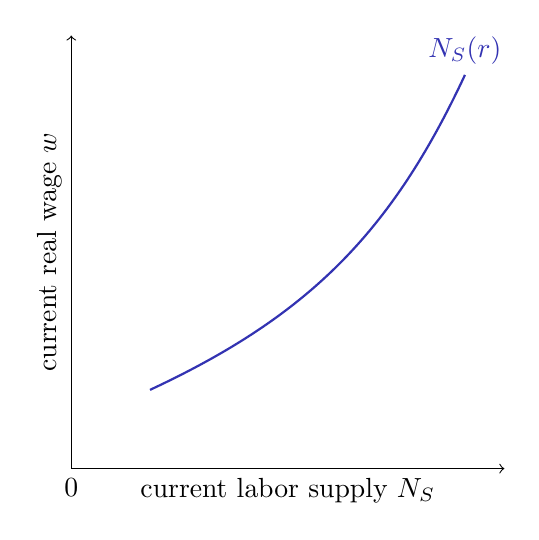
\begin{tikzpicture}
                    \pgfmathsetmacro{\x}{5};
                    \pgfmathsetmacro{\y}{5};
                    % \draw[very thin,color=gray, step=0.1] (0,0) grid (\x, \y); % gray grid
                    \draw[->] (0,0) node[below]{ $ 0 $  } -- node[below]{current labor supply $N_{S}$} (\x + 0.5,0) ;   % label x axis
                    \draw[->] (0,0) -- node[above, rotate=90]{current real wage $ w $} (0,\y + 0.5) ;   % label y axis
                    \draw[thick, blue] (1, 1) to[bend right=20] (5, 5) node[above]{$N_{S}( r )$};
                \end{tikzpicture}
            \end{figure}
        \end{column}
        \begin{column}{0.5\textwidth}
            \textbf{Assumption N1}: current labor supply $ \uparrow  $ in current wage
            \begin{itemize}
                \item Recall two effects of wage on labor:
                \begin{itemize}
                    \item income (I): $ l\uparrow, N_{S}\downarrow   $
                    \item substitution (S): $ l\downarrow, N_{S}\uparrow   $
                \end{itemize}
                \item \textbf{N1} suggests that \alert{substitution effect $ > $ income effect}
                \item data: (I) and (S) cancel out in long-run, while RBC focus on \alert{short- and medium run}!
            \end{itemize}
        \end{column}
    \end{columns}
\end{frame}

\begin{frame}{Current Labor Supply and Real Interest Rate}
\label{slide:Current_Labor_Supply_and_Real_Interest_Rate}
    \begin{columns}
        \begin{column}{0.48\textwidth}
            \begin{figure}
                \caption{\scriptsize Figure 11.2  Real Interest Rate $ \uparrow  $ Shifts the Current Labor Supply Curve to the Right}
                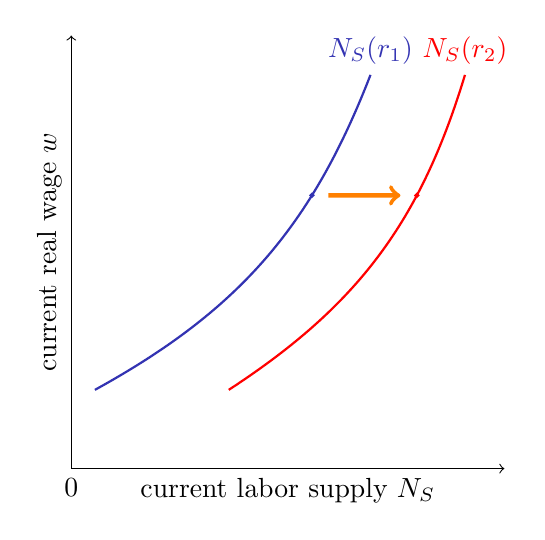
\begin{tikzpicture}
                    \pgfmathsetmacro{\x}{5};
                    \pgfmathsetmacro{\y}{5};
                    % \draw[very thin,color=gray, step=0.1] (0,0) grid (\x, \y); % gray grid
                    \draw[->] (0,0) node[below]{ $ 0 $  } -- node[below]{current labor supply $N_{S}$} (\x + 0.5,0) ;   % label x axis
                    \draw[->] (0,0) -- node[above, rotate=90]{current real wage $ w $} (0,\y + 0.5) ;   % label y axis
                    \draw[thick, blue] (0.3, 1) to[bend right=20]
                        node[pos=0.7,draw,fill=red,circle,inner sep=0pt] (a) {}
                        (3.8, 5) node[above]{$N_{S}( r_{1} )$};
                    \draw[thick, red] (2, 1) to[bend right=20]
                        node[pos=0.69,draw,fill=red,circle,inner sep=0pt] (b) {}
                        (5, 5) node[above]{$N_{S}( r_{2} )$};
                    \draw[shorten >= 5pt, shorten <= 5pt, ultra thick, orange, ->] (a) -- (b) ;
                \end{tikzpicture}
            \end{figure}
        \end{column}
        \begin{column}{0.52\textwidth}
            \textbf{Assumption N2}: current labor supply $ \uparrow  $ as real interest rate $ \uparrow  $
            \begin{itemize}
                \item can substitute \alert{intertemporally} using \textbf{both} consumption and labor
                \item \alert{relative price of future leisure in terms of current leisure}:
                    %
                    \begin{align*}
                        \frac{v'( N_{S} )}{v'( N_{S}' )}
                            & = \frac{v'( N_{S} )}{u'( C )} \times \frac{u'( C )}{u'( C' )} \times \frac{u'( C' )}{v'( N_{S}' )}
                        \\
                            & = w \times ( 1+r ) \times \frac{1}{w'}
                    \end{align*}
                    %
                \item fix $ w $ and $ w' $, $ r \uparrow  $ makes $ l $ become more costly, so $ N_{S} \uparrow  $
            \end{itemize}
        \end{column}
    \end{columns}
\end{frame}

\begin{frame}{Current Labor Supply and Wealth}
\label{slide:Current_Labor_Supply_and_Wealth}
    \begin{columns}
        \begin{column}{0.5\textwidth}
            \begin{figure}
                \caption{\scriptsize Figure 11.3 Effects of an Increase in Lifetime Wealth}
                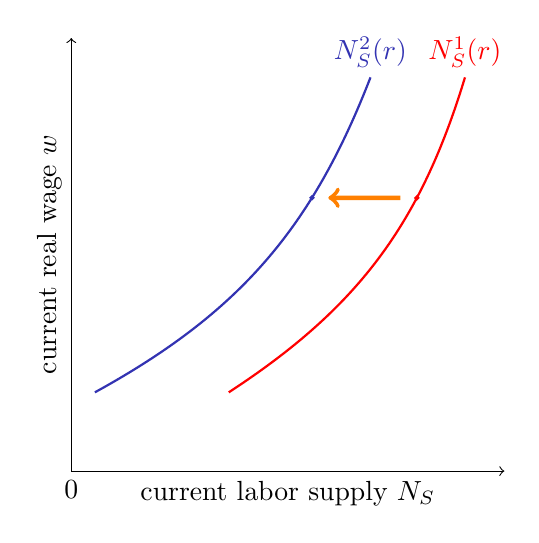
\begin{tikzpicture}
                    \pgfmathsetmacro{\x}{5};
                    \pgfmathsetmacro{\y}{5};
                    % \draw[very thin,color=gray, step=0.1] (0,0) grid (\x, \y); % gray grid
                    \draw[->] (0,0) node[below]{ $ 0 $  } -- node[below]{current labor supply $N_{S}$} (\x + 0.5,0) ;   % label x axis
                    \draw[->] (0,0) -- node[above, rotate=90]{current real wage $ w $} (0,\y + 0.5) ;   % label y axis
                    \draw[thick, blue] (0.3, 1) to[bend right=20]
                        node[pos=0.7,draw,fill=red,circle,inner sep=0pt] (a) {}
                        (3.8, 5) node[above]{$N_{S}^{2}( r )$};
                    \draw[thick, red] (2, 1) to[bend right=20]
                        node[pos=0.69,draw,fill=red,circle,inner sep=0pt] (b) {}
                        (5, 5) node[above]{$N_{S}^{1}( r )$};
                    \draw[shorten >= 5pt, shorten <= 5pt, ultra thick, orange, ->] (b) -- (a) ;
                \end{tikzpicture}
            \end{figure}
        \end{column}
        \begin{column}{0.5\textwidth}
            \textbf{Assumption N3}: current labor supply $ \downarrow  $ as lifetime wealth $ \uparrow  $
            \begin{itemize}
                \item only pure income effect on normal goods (consumption \& leisure), and thus labor decreases
            \end{itemize}
        \end{column}
    \end{columns}

\end{frame}

\begin{frame}{Summary of Effect on Labor Supply}
\label{slide:Summary_of_Effect_on_Labor_Supply}

\begin{itemize}
    \item \textbf{Assumption N1}: current labor supply $ \uparrow  $ in current wage
    \begin{itemize}
        \item $ \frac{d N_{S}}{d w} > 0 $
    \end{itemize}
    \item \textbf{Assumption N2}: current labor supply $ \uparrow  $ as real interest rate $ \uparrow  $
    \begin{itemize}
        \item $ \frac{d N_{S}}{d r} > 0 $
    \end{itemize}
    \item \textbf{Assumption N3}: current labor supply $ \downarrow  $ as lifetime wealth $ \uparrow  $
    \begin{itemize}
        \item $ \frac{d N_{S}}{d x} < 0 $, where $ x = \pi - T $.
    \end{itemize}
\end{itemize}
\alert{All statements are properties about \textbf{supply curve}, not equilibrium quantities!}
\end{frame}



\end{document}

